\section{Results}
\subsection{Inference without reionization parameter}
Since the parameter $\tau$ has a known physical degeneracy with the parameter $A_s$ \cite{HuWhite1997}, the set of six parameters was temporarily reduced to five, with $\tau$ later added back. The results of training NPSE inference models with the power spectra $C_{\ell}^{TT}$, $C_{\ell}^{EE}$, $C_{\ell}^{BB}$, and $C_{\ell}^{TE}$ in the range $0 \leq \ell \leq 2500$ are shown in Figure \ref{fig:parameters_inference}.  

\begin{figure}
    \centering
    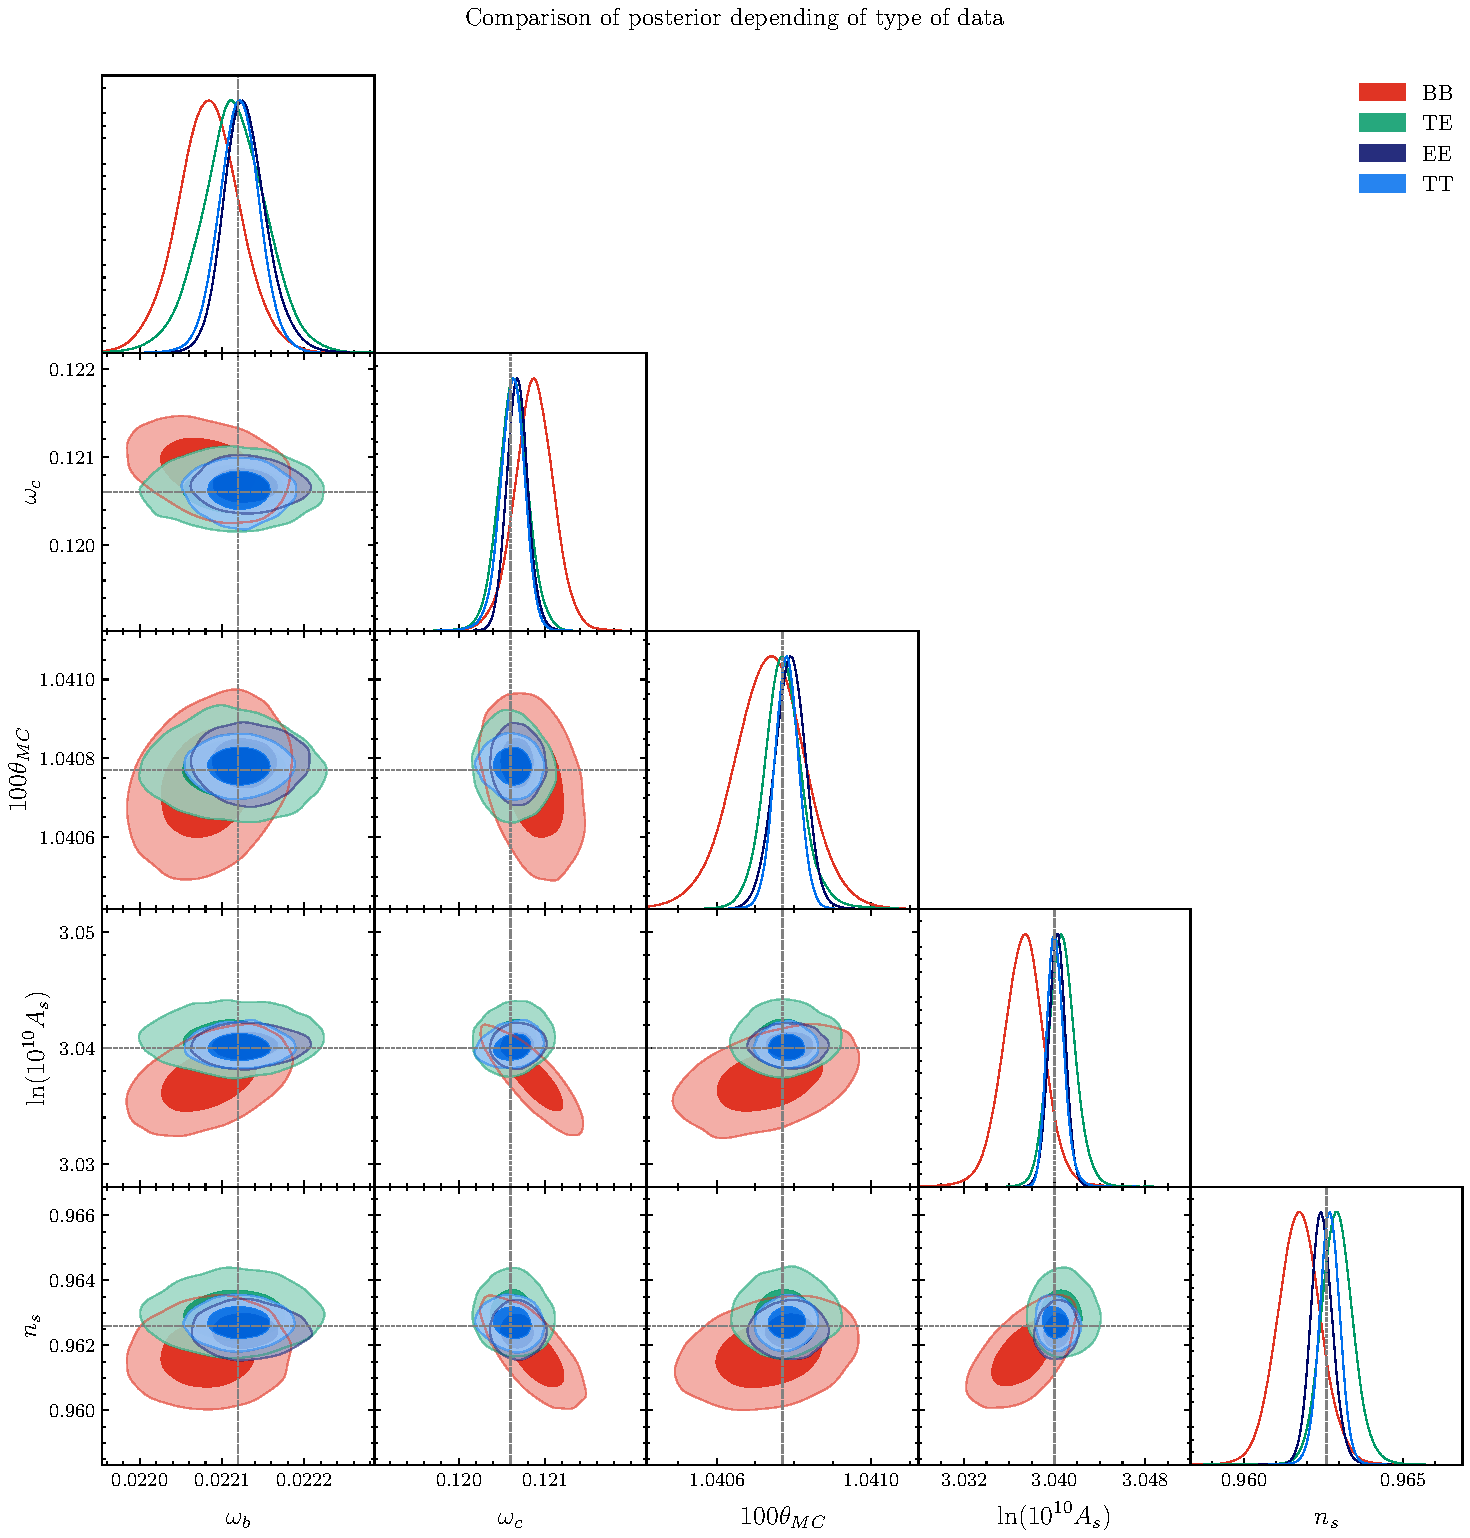
\includegraphics[scale=0.35]{img/data_comparison.pdf}
    \caption{NPSE inference models trained with 100,000 simulations of the power spectra $C_{\ell}^{TT}$, $C_{\ell}^{EE}$, $C_{\ell}^{BB}$, and $C_{\ell}^{TE}$. Each color represents a model trained with a different power spectrum. The dashed line shows the true value of the parameters.}
    \label{fig:parameters_inference}
\end{figure}

The results show how the choice of dataset ($C_{\ell}^{TT}$, $C_{\ell}^{EE}$, $C_{\ell}^{BB}$, $C_{\ell}^{TE}$) affects the posterior distributions of the selected cosmological parameters. The variation in $\omega_b$, $\omega_c$, $n_s$, $\ln(10^{10}A_s)$, and $100\theta_{MC}$ is small but non-negligible, reflecting the sensitivity of each parameter to the type of information included. In particular, the temperature and E-mode spectra (TT, EE, TE) introduce slight tensions compared to the B-mode spectrum (BB), highlighting the lack of information contained in the B-mode spectra computed only from scalar perturbations, without including primordial B-modes. Figure \ref{fig:pred_vs_obs} shows the comparison between the power spectra corresponding to the true parameters and those corresponding to a random sample from the posterior distribution obtained by training an NPSE inference model with 100,000 simulations of the $C_{\ell}^{TT}$ power spectrum.  

\subsection{Inference with reionization parameter}
When the parameter $\tau$ is included, the full set of six cosmological parameters is recovered. Figure \ref{fig:parameters_inference_tau} shows the results obtained by training the NPSE inference model with 100,000 simulations including $\tau$. This parameter introduces a clear degeneracy with $\ln(10^{10}A_s)$, which results in a broadening and a slight bias in the posterior distribution of both parameters compared to the case without $\tau$, as well as an elongation of their joint distribution.  

Moreover, the inclusion of $\tau$ produces slight variations in the posterior distributions of $n_s$ and $\omega_c$, although these remain within statistical dispersion. The temperature (TT) and polarization (EE, TE) spectra, particularly at large scales, provide the strongest sensitivity to the value of $\tau$, while the TT modes at high multipoles are unable to break the degeneracy. Consequently, this confirms the necessity of incorporating information from the first 30 multipoles of the polarization spectra (lowEE, lowTE) to improve the precision in the estimation of $\tau$ and, therefore, of $A_s$.

\begin{figure}
    \centering
    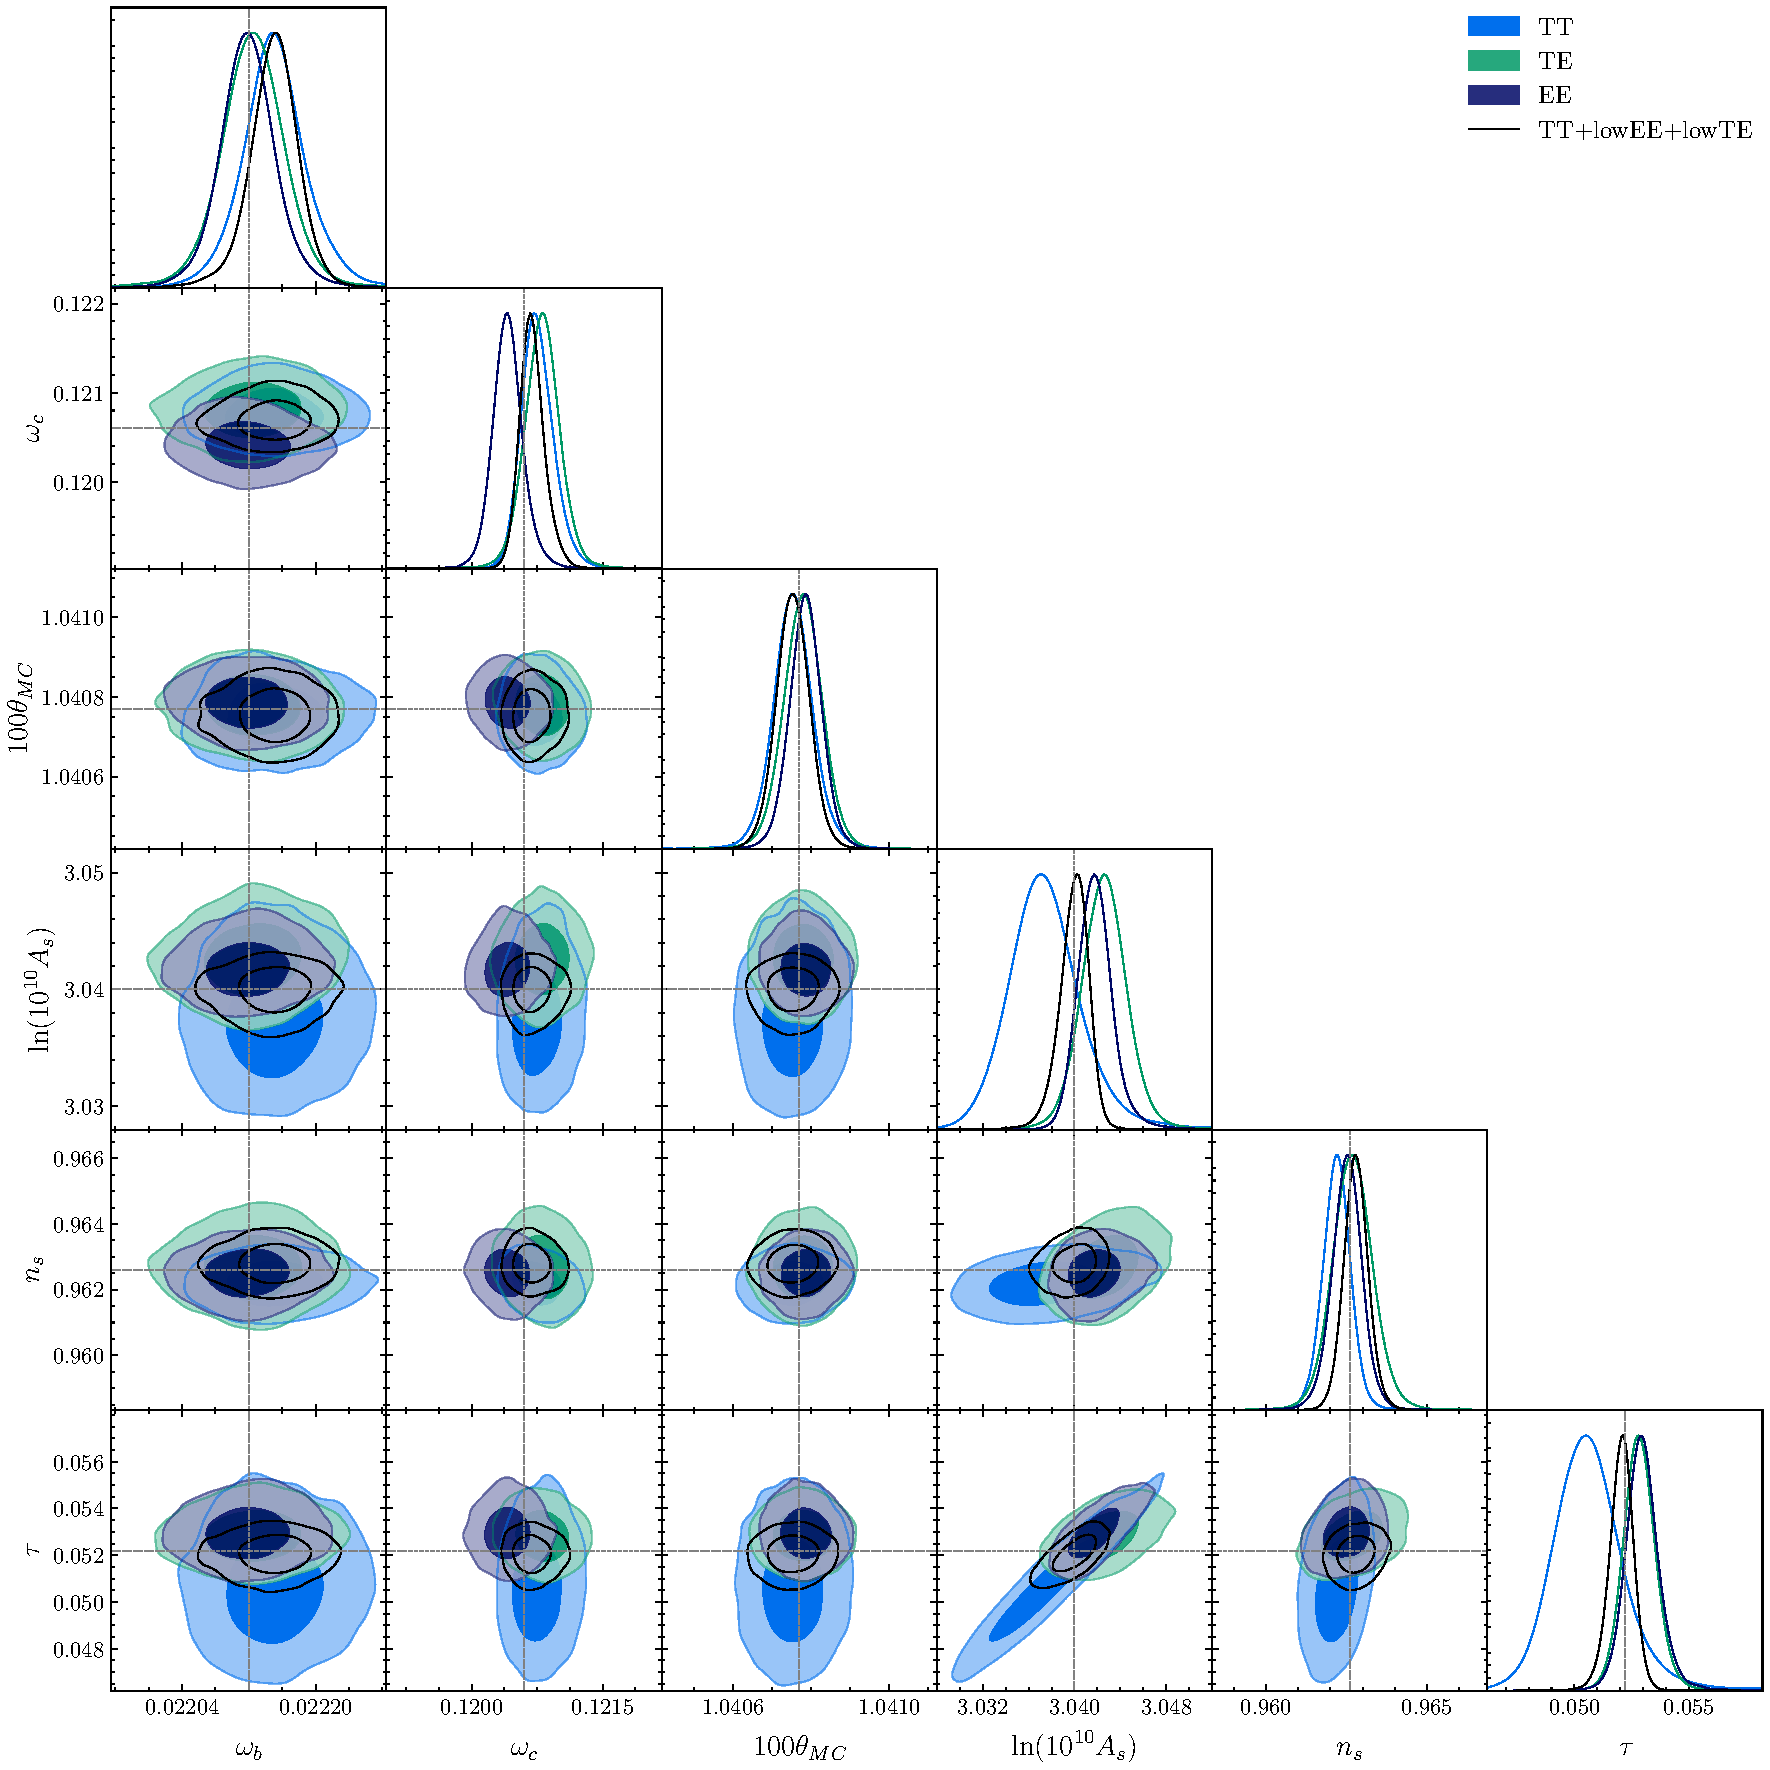
\includegraphics[scale=0.3]{img/data_comparison_tau_100000_1.pdf}
    \caption{Results of NPSE inference considering the six standard cosmological parameters, including $\tau$. The degeneracy between $\tau$ and $\ln(10^{10}A_s)$ is evident, producing a broadening of their posterior distributions. The different datasets (TT, TE, EE, and TT+lowEE+lowTE) highlight the importance of including low-multipole information to constrain the value of $\tau$.}
    \label{fig:parameters_inference_tau}
\end{figure}

\subsection{Adding Noise}
To approximate more realistic observational conditions, noise is introduced into the simulations of the power spectra $C_{\ell}^{TT}$. We mainly consider two sources: the instrumental noise of the experiment and the partial sky coverage, which adds additional cosmic variance. First, instrumental noise is incorporated into the theoretical spectra using a model based on the angular resolution of the instrument (\(\theta_{\text{fwhm}}\)) and the pixel sensitivity (\(\sigma_T\)) \cite{noiseCole}. The instrumental noise term \(N_\ell^{\mathrm{TT}}\), which is added to the theoretical power spectrum \(C_\ell\), is defined as:

\begin{equation}
N_\ell^{\mathrm{TT}} = \left(\theta_{\text{fwhm}} \cdot \sigma_T \right)^2 \exp\left[ \ell (\ell + 1) \frac{\theta_{\text{fwhm}}^2}{8 \ln 2} \right],
\end{equation}

where \(\theta_{\text{fwhm}}\) is expressed in radians. This expression models the sky smoothing due to the finite resolution of the instrument.

Subsequently, the observation of a partial sky is simulated, considering that only a fraction \(f_{\text{sky}} < 1\) of the full sky is measured. As a result, the observable estimator of \(C_\ell\), denoted \(\hat{C}_\ell\), becomes a random variable whose dispersion depends on \(f_{\text{sky}}\). For low multipoles (\(\ell < \ell_{\text{transition}}\)), this variance is modeled through a scaled chi-squared distribution:

\begin{equation}
\hat{C}_\ell = \frac{1}{\nu_\ell} \sum_{i=1}^{\nu_\ell} X_i^2, \quad X_i \sim \mathcal{N}(0, \sqrt{C_\ell}),
\end{equation}

where \(\nu_\ell = \text{round}(f_{\text{sky}} \cdot (2\ell + 1))\) represents the effective number of degrees of freedom. This formulation correctly captures the statistical dispersion of the estimator when the number of available modes is limited. For high multipoles (\(\ell \geq \ell_{\text{transition}}\)), it is assumed that the estimator can be approximated by a normal distribution centered on \(C_\ell\) with variance:

\begin{equation}
\hat{C}_\ell \sim \mathcal{N}\left(C_\ell, \frac{2 C_\ell^2}{f_{\text{sky}} (2\ell + 1)} \right).
\end{equation}

This Gaussian approximation is valid thanks to the central limit theorem, since in this regime the number of available modes is sufficiently large.

\begin{figure}
    \centering
    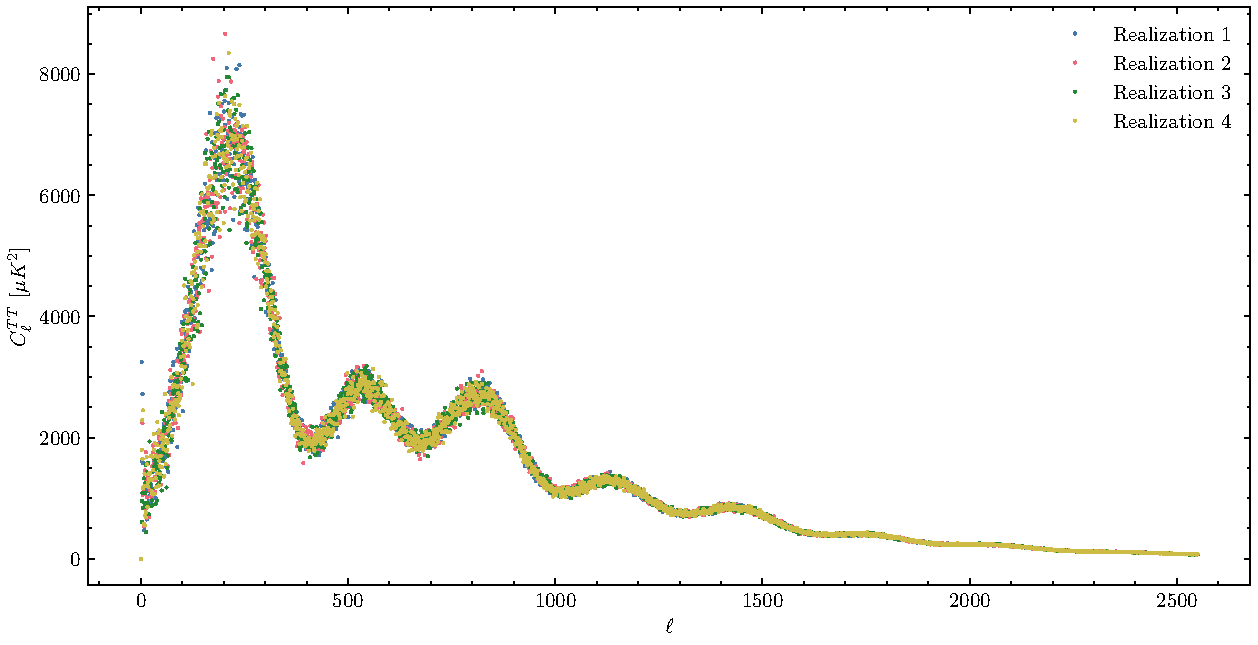
\includegraphics[scale=0.41]{img/grafico.pdf}
    \caption{Multiple realizations of a power spectrum for the same combination of cosmological parameters, including instrumental noise and the effect of partial sky coverage. Each color represents a different realization.}
    \label{fig:realizations_noise}
\end{figure}

To capture the randomness introduced by noise in the power spectra, multiple realizations of each combination of cosmological parameters were generated in the training set \cite{novaes}. Each cosmology was simulated several times, applying instrumental noise and the variance associated with partial sky coverage, so that the model can learn the natural dispersion of the observables due to these sources of uncertainty. This approach allows the inference model not only to learn the average values of the spectra, but also to internalize the statistical variability caused by noise. In this way, the posterior predictions more realistically reflect the uncertainty expected in real observational data.

Figure \ref{fig:realizations_noise} shows an example of multiple realizations of the power spectrum for the same cosmology, where each colored line represents a different realization. It can be observed how noise produces significant variations in the spectrum, especially at scales where instrumental noise and partial sky coverage have the greatest effect.

\begin{figure}
    \centering
    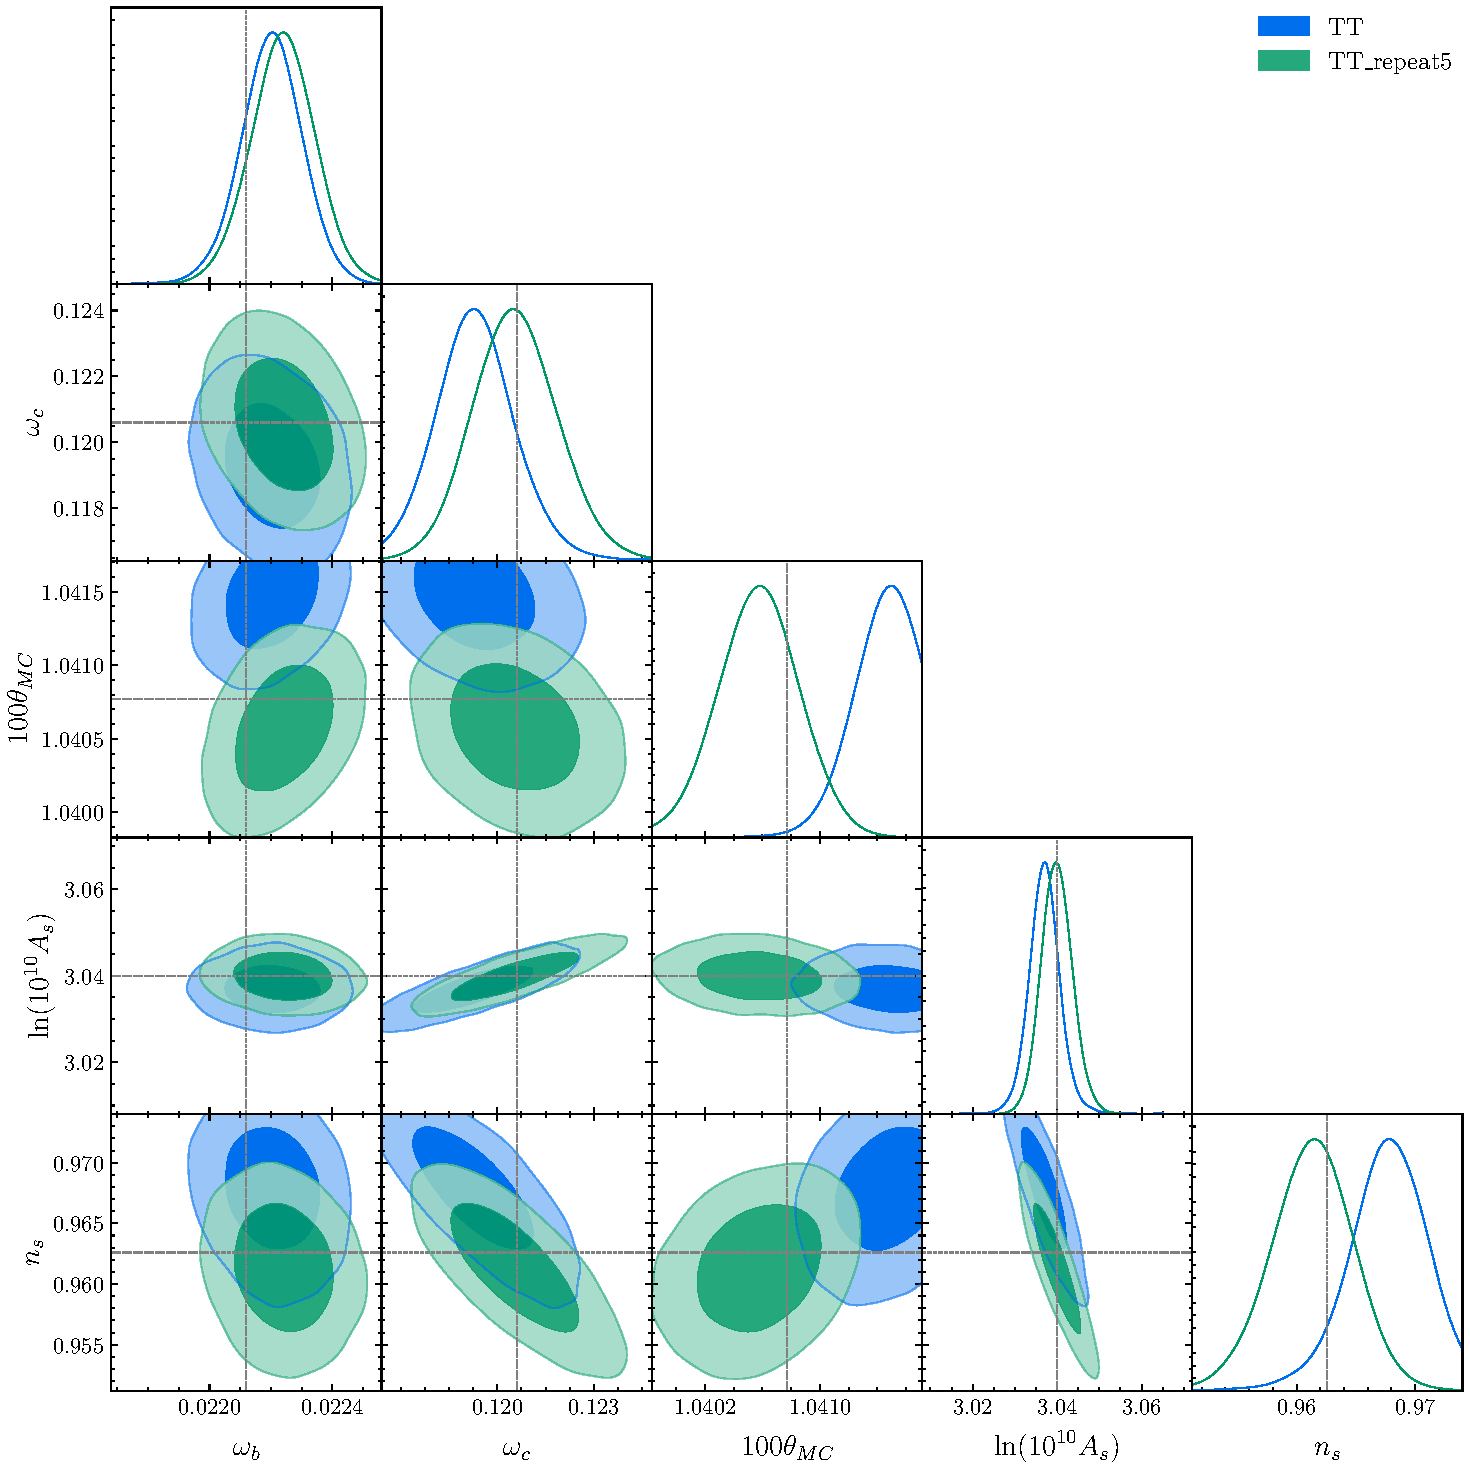
\includegraphics[scale=0.35]{img/01_repeat_noise_comparison_100000.pdf}
    \caption{Inference of cosmological parameters from the TT power spectrum. The model training without additional realizations (\texttt{TT}) is compared to the case with five noisy realizations per cosmology (\texttt{TT repeat5}).}
    \label{fig:inference_with_noise}
\end{figure}

Figure \ref{fig:inference_with_noise} presents the posterior distributions of cosmological parameters obtained under two training schemes. In the case without additional realizations (blue plot), the distributions appear narrower, reflecting an underestimation of the true uncertainty associated with the data. In contrast, when five noisy realizations per cosmology are included in the training (green plot), the posteriors are more consistently centered and capture more faithfully the dispersion induced by instrumental noise.

Although the scheme with realizations still shows residual artificial degeneracies and biases, the results are significantly improved compared to the scheme without realizations. Most parameters exhibit intervals that are closer to the expected statistical variability, indicating that the model, when exposed to multiple realizations, better internalizes the stochastic nature of the data and avoids an overconfident characterization of the posteriors.









